\chapter{Einführung}

Mittels eines Polygonnetzes lassen sich Flächen verschiedener Formen beschreiben. 
Meist wird ein sog. Kontrollnetz verwendet, welches von einem Modellierer erstellt wird.
Dieses wird dann durch computergestützte Verarbeitung verfeinert, um eine glatte Fläche zu erzeugen.
Hierbei stellt sich die Herausforderung, mit möglichst wenigen Polygonen im Kontrollnetz eine glatte Oberfläche erzeugen zu können.
Ein kleines Kontrollnetz spart Speicherplatz und senkt die Komplexität bei Änderungen im Netz.
Ein in der Computergrafik häufig verwendeter Ansatz zur Berechnung von glatten Oberflächen aus einem Kontrollnetz, ist die Anwendung von Unterteilungsalgorithmen.
Hier soll insbesondere der Algorithmus von Catmull-Clark erwähnt werden.
Pixar verwendet diesen für die Entwicklung von animierten Filmen (siehe \autoref{fig:subdiv_einleitung}).

\begin{figure}
  \centering
  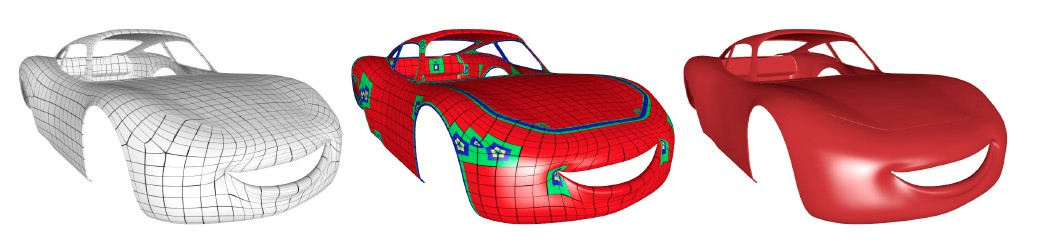
\includegraphics[width=\textwidth]{content/media/sd_einleitung.jpg}
  \caption{Anwendung von Catmull-Clark \cite{niessner2012feature}}
  \label{fig:subdiv_einleitung}
\end{figure}


Das Projekt \emph{SubVis} setzt sich zum Ziel ein Programm zu entwickeln, das einige Unterteilungsalgorithmen implementiert und visualisiert. 
Dabei soll einerseits das Kontrollnetz (Polygonnetz) als auch die durch Anwendung von Unterteilungsalgorithmen entstehende Limesfläche dargestellt werden.
Dies dient dazu, die Vielzahl an Algorithmen an einem Ort zu bündeln und über eine schlanke, übersichtliche Anwendung zu Verfügung zu stellen.
Hiervon sollen insbesondere Studenten und andere interessierte Personen profitieren, die sich mit der Thematik auseinandersetzen möchten.
Der modulare Aufbau und eine gute Dokumentation sollen nachfolgenden Projekten (Abschlussarbeiten, Teamprojekte, etc.) die Möglichkeit geben, die Anwendung weiter zu entwickeln bzw. zu erweitern.

Es wird nachfolgend eine kurze Einführung in die Thematik gegeben, gefolgt von der Evaluierung verschiedener Tools und Bibliotheken. 
Danach folgt eine Beschreibung des geplanten Programms \emph{SubVis}.
Abschließend wird der bisherige Projektverlauf und ein Ausblick für das kommende Semester dargelegt.